%!TeX root=../pridetop.tex

\chapter[Chapter \thechapter]{}
	
	\begin{figure}[t!]
\centering
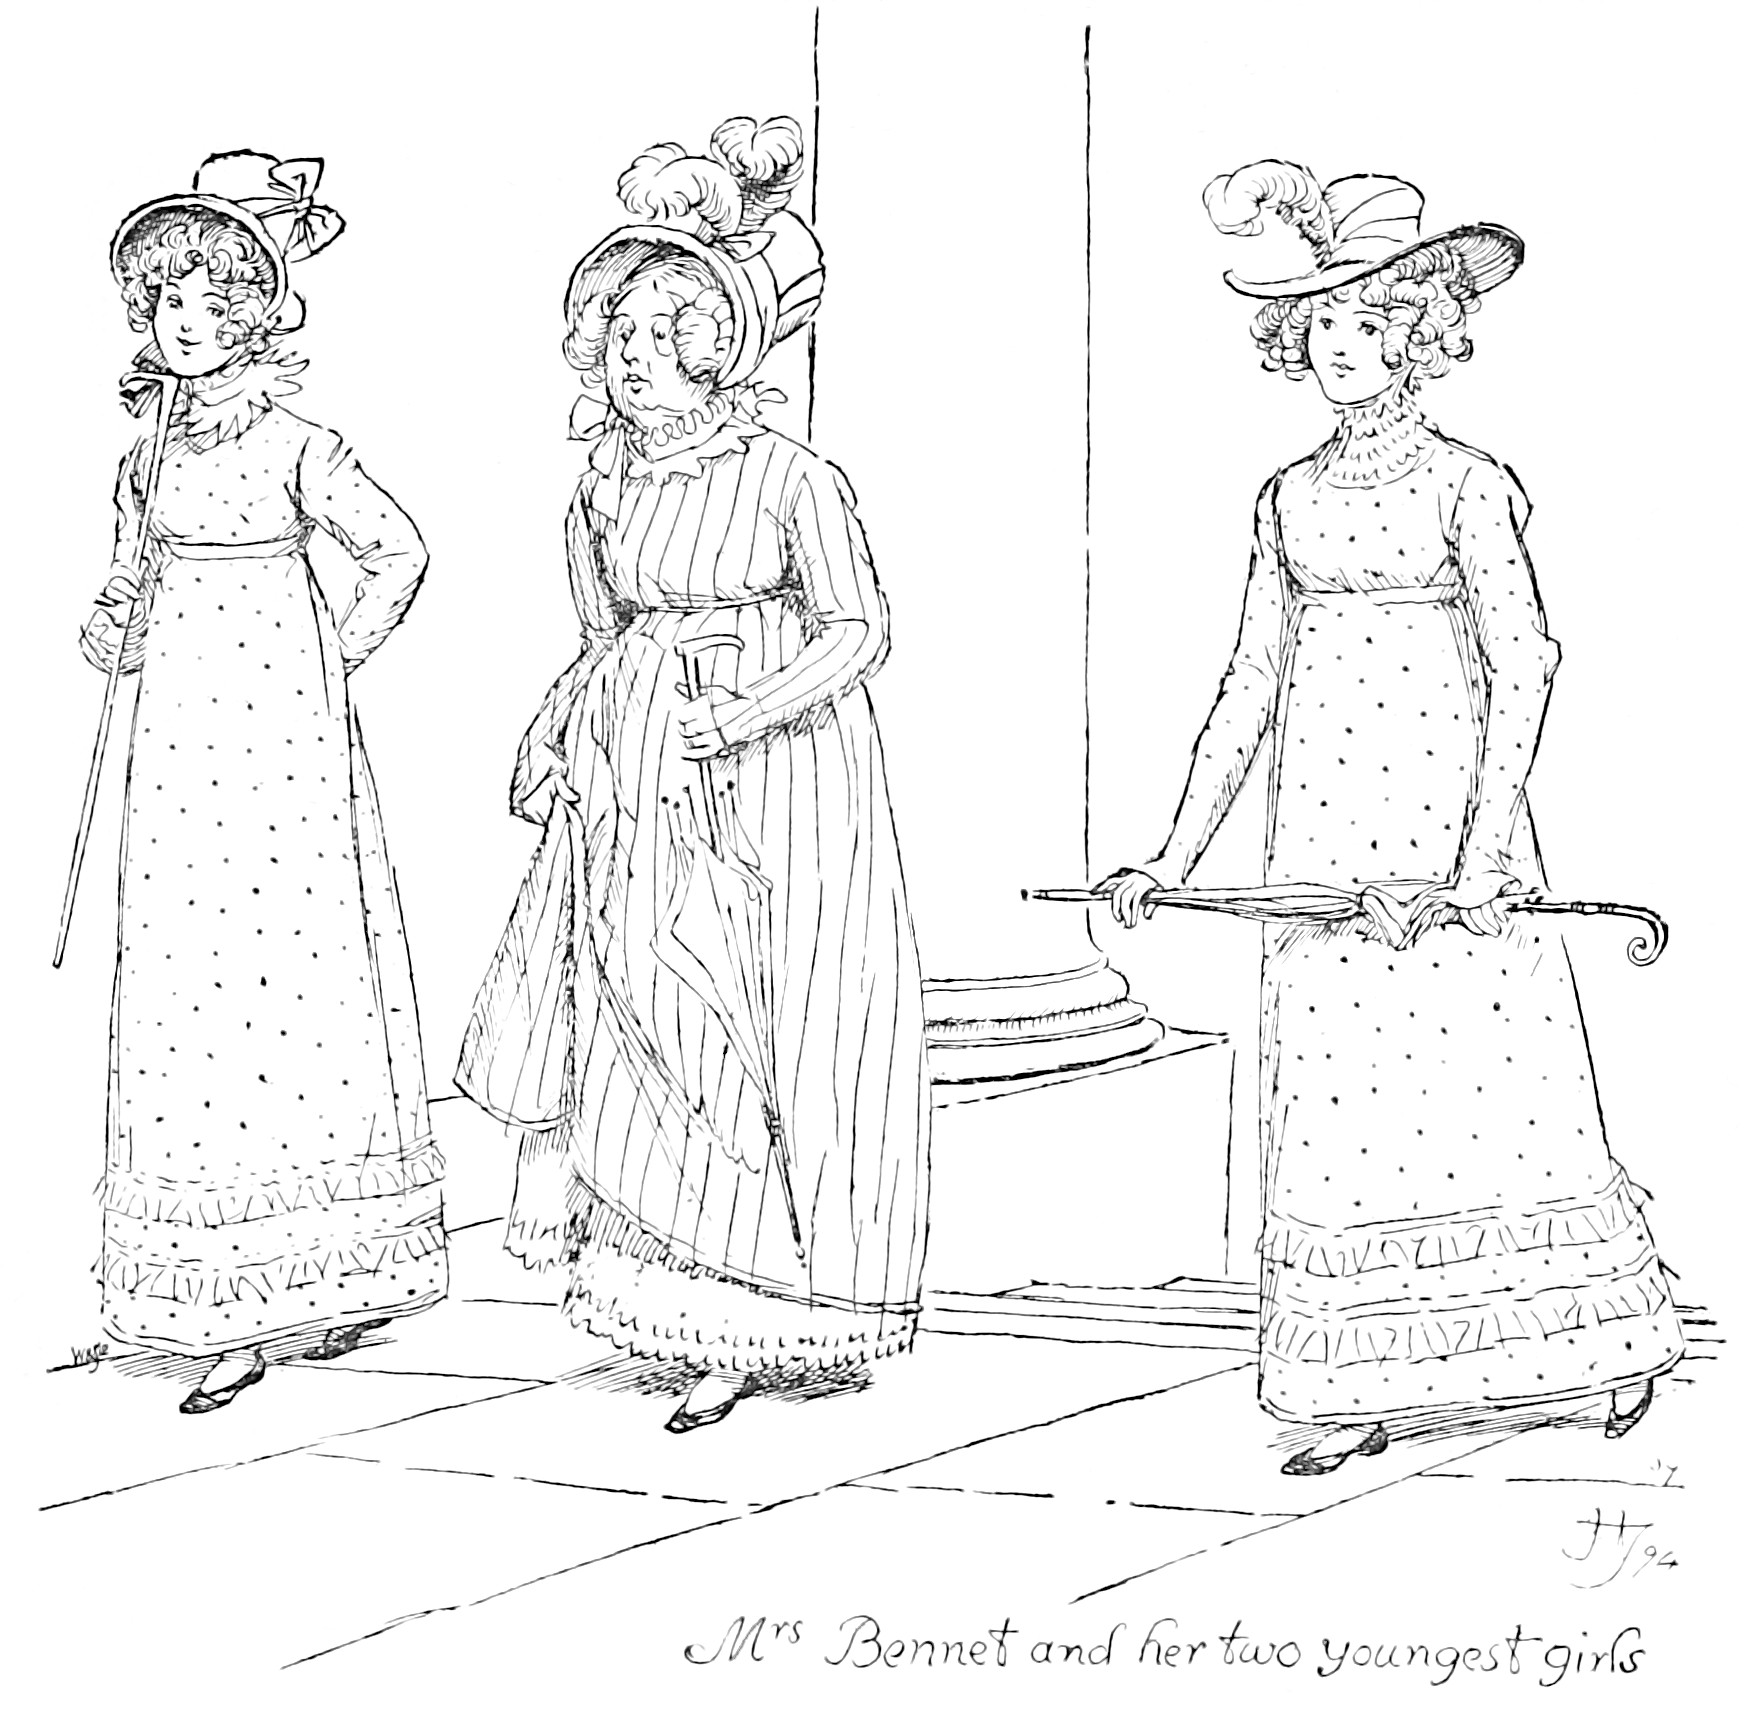
\includegraphics[width=.8\linewidth]{9bennetgirls}
\captionlistentry{Mrs Bennet and her two youngest girls}
\end{figure}

	\lettrine[lines=6,image=true]{initials/chap9e}{lizabeth}  passed the chief of the night in her sister's room, and in the morning had the pleasure of being able to send a tolerable answer to the inquiries which she very early received from Mr Bingley by a housemaid, and some time afterwards from the two elegant ladies who waited on his sisters. In spite of this amendment, however, she requested to have a note sent to Longbourn, desiring her mother to visit Jane, and form her own judgment of her situation. The note was immediately despatched, and its contents as quickly complied with. Mrs Bennet, accompanied by her two youngest girls, reached Netherfield soon after the family breakfast.



Had she found Jane in any apparent danger, Mrs Bennet would have been very miserable; but being satisfied on seeing her that her illness was not alarming, she had no wish of her recovering immediately, as her restoration to health would probably remove her from Netherfield. She would not listen, therefore, to her daughter's proposal of being carried home; neither did the apothecary, who arrived about the same time, think it at all advisable. After sitting a little while with Jane, on Miss Bingley's appearance and invitation, the mother and three daughters all attended her into the breakfast parlour. Bingley met them with hopes that Mrs Bennet had not found Miss Bennet worse than she expected.

»Indeed I have, sir,« was her answer. »She is a great deal too ill to be moved. Mr Jones says we must not think of moving her. We must trespass a little longer on your kindness.«

»Removed!« cried Bingley. »It must not be thought of. My sister, I am sure, will not hear of her removal.«

»You may depend upon it, madam,« said Miss Bingley, with cold civility, »that Miss Bennet shall receive every possible attention while she remains with us.«

Mrs Bennet was profuse in her acknowledgments.

»I am sure,« she added, »if it was not for such good friends, I do not know what would become of her, for she is very ill indeed, and suffers a vast deal, though with the greatest patience in the world, which is always the way with her, for she has, without exception, the sweetest temper I ever met with. I often tell my other girls they are nothing to \textit{her}. You have a sweet room here, Mr Bingley, and a charming prospect over that gravel walk. I do not know a place in the country that is equal to Netherfield. You will not think of quitting it in a hurry, I hope, though you have but a short lease.«

»Whatever I do is done in a hurry,« replied he; »and therefore if I should resolve to quit Netherfield, I should probably be off in five minutes. At present, however, I consider myself as quite fixed here.«

»That is exactly what I should have supposed of you,« said Elizabeth.

»You begin to comprehend me, do you?« cried he, turning towards her.

»Oh yes—I understand you perfectly.«

»I wish I might take this for a compliment; but to be so easily seen through, I am afraid, is pitiful.«

»That is as it happens. It does not necessarily follow that a deep, intricate character is more or less estimable than such a one as yours.«

»Lizzy,« cried her mother, »remember where you are, and do not run on in the wild manner that you are suffered to do at home.«

»I did not know before,« continued Bingley, immediately, »that you were a studier of character. It must be an amusing study.«

»Yes; but intricate characters are the \textit{most} amusing. They have at least that advantage.«

»The country,« said Darcy, »can in general supply but few subjects for such a study. In a country neighbourhood you move in a very confined and unvarying society.«

»But people themselves alter so much, that there is something new to be observed in them for ever.«

»Yes, indeed,« cried Mrs Bennet, offended by his manner of mentioning a country neighbourhood. »I assure you there is quite as much of \textit{that} going on in the country as in town.«

Everybody was surprised; and Darcy, after looking at her for a moment, turned silently away. Mrs Bennet, who fancied she had gained a complete victory over him, continued her triumph,—

»I cannot see that London has any great advantage over the country, for my part, except the shops and public places. The country is a vast deal pleasanter, is not it, Mr Bingley?«

»When I am in the country,« he replied, »I never wish to leave it; and when I am in town, it is pretty much the same. They have each their advantages, and I can be equally happy in either.«

»Ay, that is because you have the right disposition. But that gentleman,« looking at Darcy, »seemed to think the country was nothing at all.«

»Indeed, mamma, you are mistaken,« said Elizabeth, blushing for her mother. »You quite mistook Mr Darcy. He only meant that there was not such a variety of people to be met with in the country as in town, which you must acknowledge to be true.«

»Certainly, my dear, nobody said there were; but as to not meeting with many people in this neighbourhood, I believe there are few neighbourhoods larger. I know we dine with four-and-twenty families.«

Nothing but concern for Elizabeth could enable Bingley to keep his countenance. His sister was less delicate, and directed her eye towards Mr Darcy with a very expressive smile. Elizabeth, for the sake of saying something that might turn her mother's thoughts, now asked her if Charlotte Lucas had been at Longbourn since \textit{her} coming away.

»Yes, she called yesterday with her father. What an agreeable man Sir William is, Mr Bingley—is not he? so much the man of fashion! so genteel and so easy! He has always something to say to everybody. \textit{That} is my idea of good breeding; and those persons who fancy themselves very important and never open their mouths quite mistake the matter.«

»Did Charlotte dine with you?«

»No, she would go home. I fancy she was wanted about the mince-pies. For my part, Mr Bingley, \textit{I} always keep servants that can do their own work; \textit{my} daughters are brought up differently. But everybody is to judge for themselves, and the Lucases are a very good sort of girls, I assure you. It is a pity they are not handsome! Not that \textit{I} think Charlotte so \textit{very} plain; but then she is our particular friend.«

»She seems a very pleasant young woman,« said Bingley.

»Oh dear, yes; but you must own she is very plain. Lady Lucas herself has often said so, and envied me Jane's beauty. I do not like to boast of my own child; but to be sure, Jane—one does not often see anybody better looking. It is what everybody says. I do not trust my own partiality. When she was only fifteen there was a gentleman at my brother Gardiner's in town so much in love with her, that my sister-in-law was sure he would make her an offer before we came away. But, however, he did not. Perhaps he thought her too young. However, he wrote some verses on her, and very pretty they were.«

»And so ended his affection,« said Elizabeth, impatiently. »There has been many a one, I fancy, overcome in the same way. I wonder who first discovered the efficacy of poetry in driving away love!«

»I have been used to consider poetry as the \textit{food} of love,« said Darcy.

»Of a fine, stout, healthy love it may. Everything nourishes what is strong already. But if it be only a slight, thin sort of inclination, I am convinced that one good sonnet will starve it entirely away.«

Darcy only smiled; and the general pause which ensued made Elizabeth tremble lest her mother should be exposing herself again. She longed to speak, but could think of nothing to say; and after a short silence Mrs Bennet began repeating her thanks to Mr Bingley for his kindness to Jane, with an apology for troubling him also with Lizzy. Mr Bingley was unaffectedly civil in his answer, and forced his younger sister to be civil also, and say what the occasion required. She performed her part, indeed, without much graciousness, but Mrs Bennet was satisfied, and soon afterwards ordered her carriage. Upon this signal, the youngest of her daughters put herself forward. The two girls had been whispering to each other during the whole visit; and the result of it was, that the youngest should tax Mr Bingley with having promised on his first coming into the country to give a ball at Netherfield.

Lydia was a stout, well-grown girl of fifteen, with a fine complexion and good-humoured countenance; a favourite with her mother, whose affection had brought her into public at an early age. She had high animal spirits, and a sort of natural \newline self-consequence, which the attentions of the officers, to whom her uncle's good dinners and her own easy manners recommended her, had increased into assurance. She was very equal, therefore, to address Mr Bingley on the subject of the ball, and abruptly reminded him of his promise; adding, that it would be the most shameful thing in the world if he did not keep it. His answer to this sudden attack was delightful to her mother's ear.

»I am perfectly ready, I assure you, to keep my engagement; and, when your sister is recovered, you shall, if you please, name the very day of the ball. But you would not wish to be dancing while she is ill?«

Lydia declared herself satisfied. »Oh yes—it would be much better to wait till Jane was well; and by that time, most likely, Captain Carter would be at Meryton again. And when you have given \textit{your} ball,« she added, »I shall insist on their giving one also. I shall tell Colonel Forster it will be quite a shame if he does not.«

Mrs Bennet and her daughters then departed, and Elizabeth returned instantly to Jane, leaving her own and her relations' behaviour to the remarks of the two ladies and Mr Darcy; the latter of whom, however, could not be prevailed on to join in their censure of \textit{her}, in spite of all Miss Bingley's witticisms on \textit{fine eyes}.